\setchapterimage[3.5cm]{mma/crab-page}
\setchapterpreamble[u]{\margintoc}
\chapter{Multi-Messenger Astronomy}
\labch{theory}
\begin{fquote}[William Shakespeare][Hamlet][1556] Though this be madness, yet there is method in it.
\end{fquote}

Multi-wavelength astronomy seeks to understand the universe through correlations between photons of different energies. Multi-messenger astronomy expands this concept to incorporate information from non-photon messengers, namely cosmic rays, gravitational waves and neutrinos. Each messenger provides a unique view of astrophysical processes in objects.

\section{Photons}

\begin{marginfigure}
	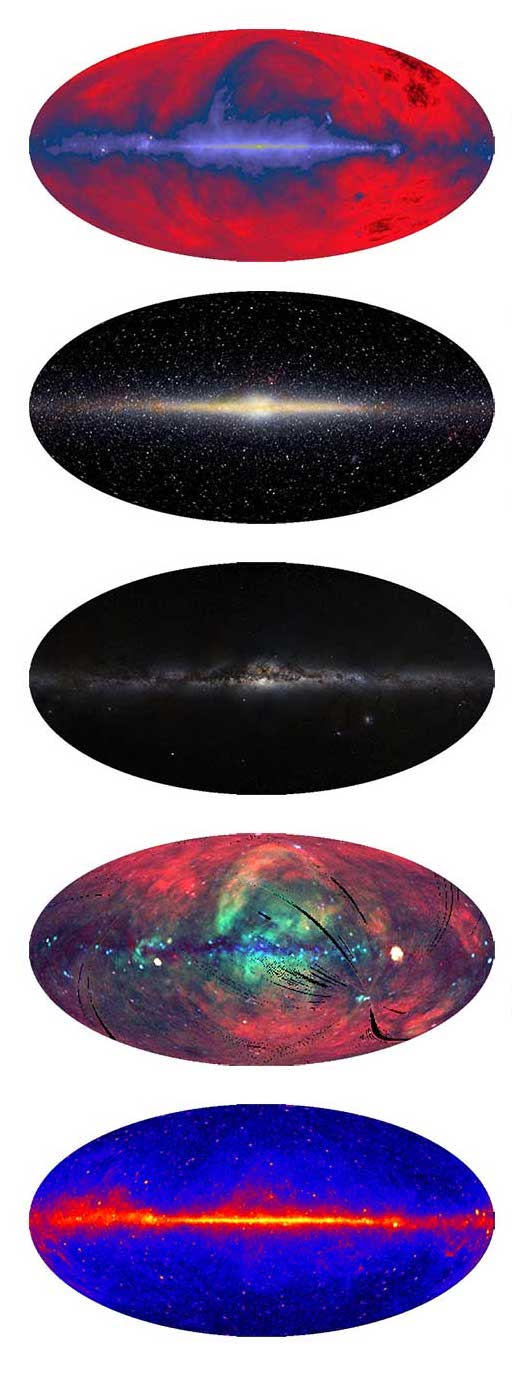
\includegraphics{mma/multiwavelength_sky_full}
	\caption{The sky, in galactic coordinates. From top: radio, infra-red, optical, X-ray and gamma-ray. Credit: NASA}
	\label{fig:mwsky}
\end{marginfigure}

Photon astronomy, in particular that in optical wavelengths, is the oldest branch of astronomy. As clear in Figure \ref{fig:mwsky}, our own galaxy is the most obvious structure at all wavelengths. The different pictures of the galaxy are also noteworthy. One example is dust extinction obscuring a large portion of the optical emission (middle panel), but  which is reprocessed to yield a particularly clear infra-red image (upper middle panel). This is an illustration of one broader principle, that interpolation between different photon energies can reveal .

In general, photon emission can be divided into two broad classes, \emph{thermal emission}
 and \emph{non-thermal emission}. Thermal emission is approximate black-bodies, and produces characteristic spectra. Non-thermal emission arises from particle acceleration, and is typically characterised by power-law emission. Objects can have both components. Thermal emission is typically centered in IR, optical or UV wavelengths, while non-thermal emission is typically manifested in both low energies (radio) and high-energies (hard X-rays and gamma-rays).
 
 \subsection{Thermal Photons}

 \subsection{Non-thermal Photons}
 
 \subsection{Spectroscopy}
 
While photon observations are typically integrated over relatively-wide 

\section{Cosmic Rays}

\emph{Cosmic Rays} were first discovered by Victor Hess in 1912 \sidecite{Hess:1912srp}. The name itself is a misnomer, as they are in fact charged particles. Being charged particles, they are deflected by magnetic fields, and it is thus challenging to determine where they originate from.

An industry of experiments has since developed to measure the composition and spectrum of Cosmic Rays, as illustrated in Figure \ref{fig:CR_spectrum}. The data is well-described by an unbroken power-law up to $\sim$1 PeV, beyond which there is a spectral softening known as \emph{the knee}. This softer spectrum continues before undergoing a hardening, known as the \emph{ankle}. There is then evidence of a high-energy cutoff, sometimes dubbed \emph{the second knee} in a case of metaphor-stretching.

\begin{figure}[!ht]
	\centering 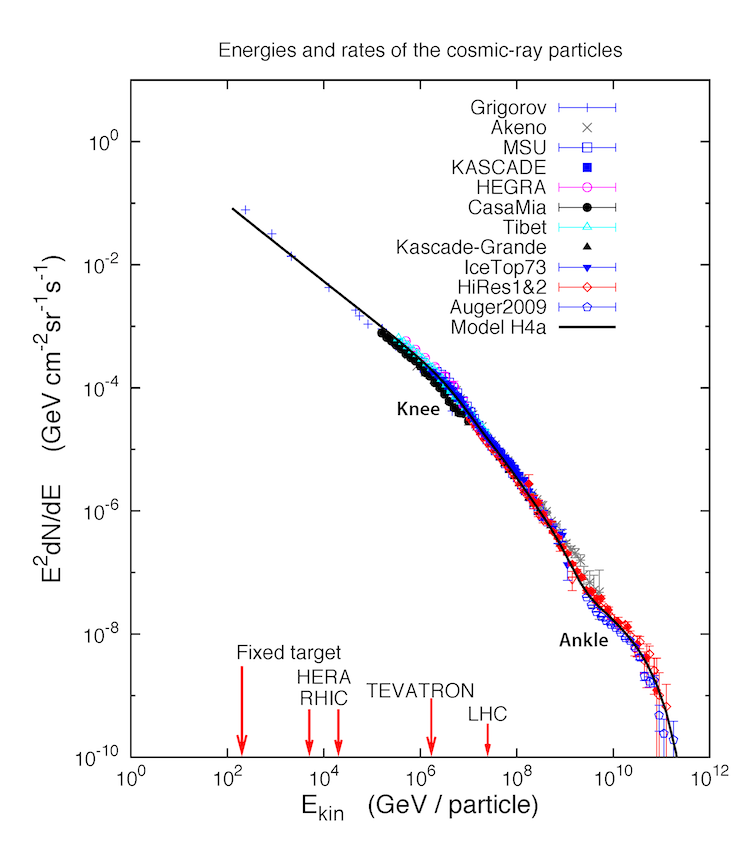
\includegraphics{mma/CRspectrum750}
	\caption{Cosmic Ray spectrum above 100 GeV, from x (icecube).}
	\label{fig:CR_spectrum}
\end{figure}

The knee is typically identified as the point at which cosmic rays transition from being predominantly galactic to extragalactic, with the ankle component being fully extragalactic. The origin of the high-energy cutoff is unclear, and the corresponding flux is so low that detector arrays must be several hundred square kilometers to study this regime with high statistics. As of 2020, this is primarily studied by the \emph{Pierre Auger Detector} and \emph {Telescope Array} detector. This regime is particularly interesting, because it is the point at which the GZK... mechanism 

UHECRs

\begin{equation}
p + \gamma_{CMB} \rightarrow \Delta^{+} \rightarrow n + \pi^{+}
\label{eq:GZK_pip}
\end{equation}
\begin{equation}
p + \gamma_{CMB} \rightarrow \Delta^{+} \rightarrow p + \pi^{0}
\label{eq:GZK_pi0}
\end{equation}

Equations \ref{eq:GZK_pip} and \ref{eq:GZK_pi0} would lead to a cutoff, in which pion production would suppress ultra-high energies above a threshold energy set by the mass of the $\Delta^{+}$ resonance. Attenuation would not occur for nearby cosmic ray sources, so the presence of such a cutoff would be evidence of an \emph{an extragalatic origin} for UHECRs. However, the \emph{Cosmic Ray Composition} determines the exact threshold for the GZK cutoff, with heavier comsic rays experiencing a much higher? threshold. There is thus much focus on understanding whether UHECRs are proton-dominated or Iron-dominated, with TA data supporting the former and PAO data supporting the latter. A joint working group concluded that these results are not in tension, once systematic uncertainties are accounted for. In summary, it appears that a definitive confirmation of a cutoff compatible with the GZK mechanism remains out of reach of present-generation instruments.

An alternative explanation for any apparent cutoff is that sources of UHECRs simply cannot accelerate particles beyond certain energies due to physical constraints. In general, any cosmic ray accelerator must at a minimum satisfy the \emph{Hillas Criterion} that any particle can be contained during the acceleration process \sidecite{1984ARA&A..22..425H}. This can be calculated by equating the Lamour Radius of a particle with the physical size of an accelerator:

Enu?

\begin{equation}
\frac{E_{\textup{max}}}{\textup{PeV}} \approx
1600 \times \frac{B}{\textup{Gauss}} \times \frac{R}{10^{16} \textup{cm}} \times
\beta Z
\label{eq:hillas}
\end{equation}

Equation \ref{eq:hillas} leads to a constraint on minimal magnetic field strength and source extension, which can be illustrated by a \emph{Hillas Plot} such as that in Figure \ref{fig:hillas_plot}.

\begin{figure}[!ht]
	\centering 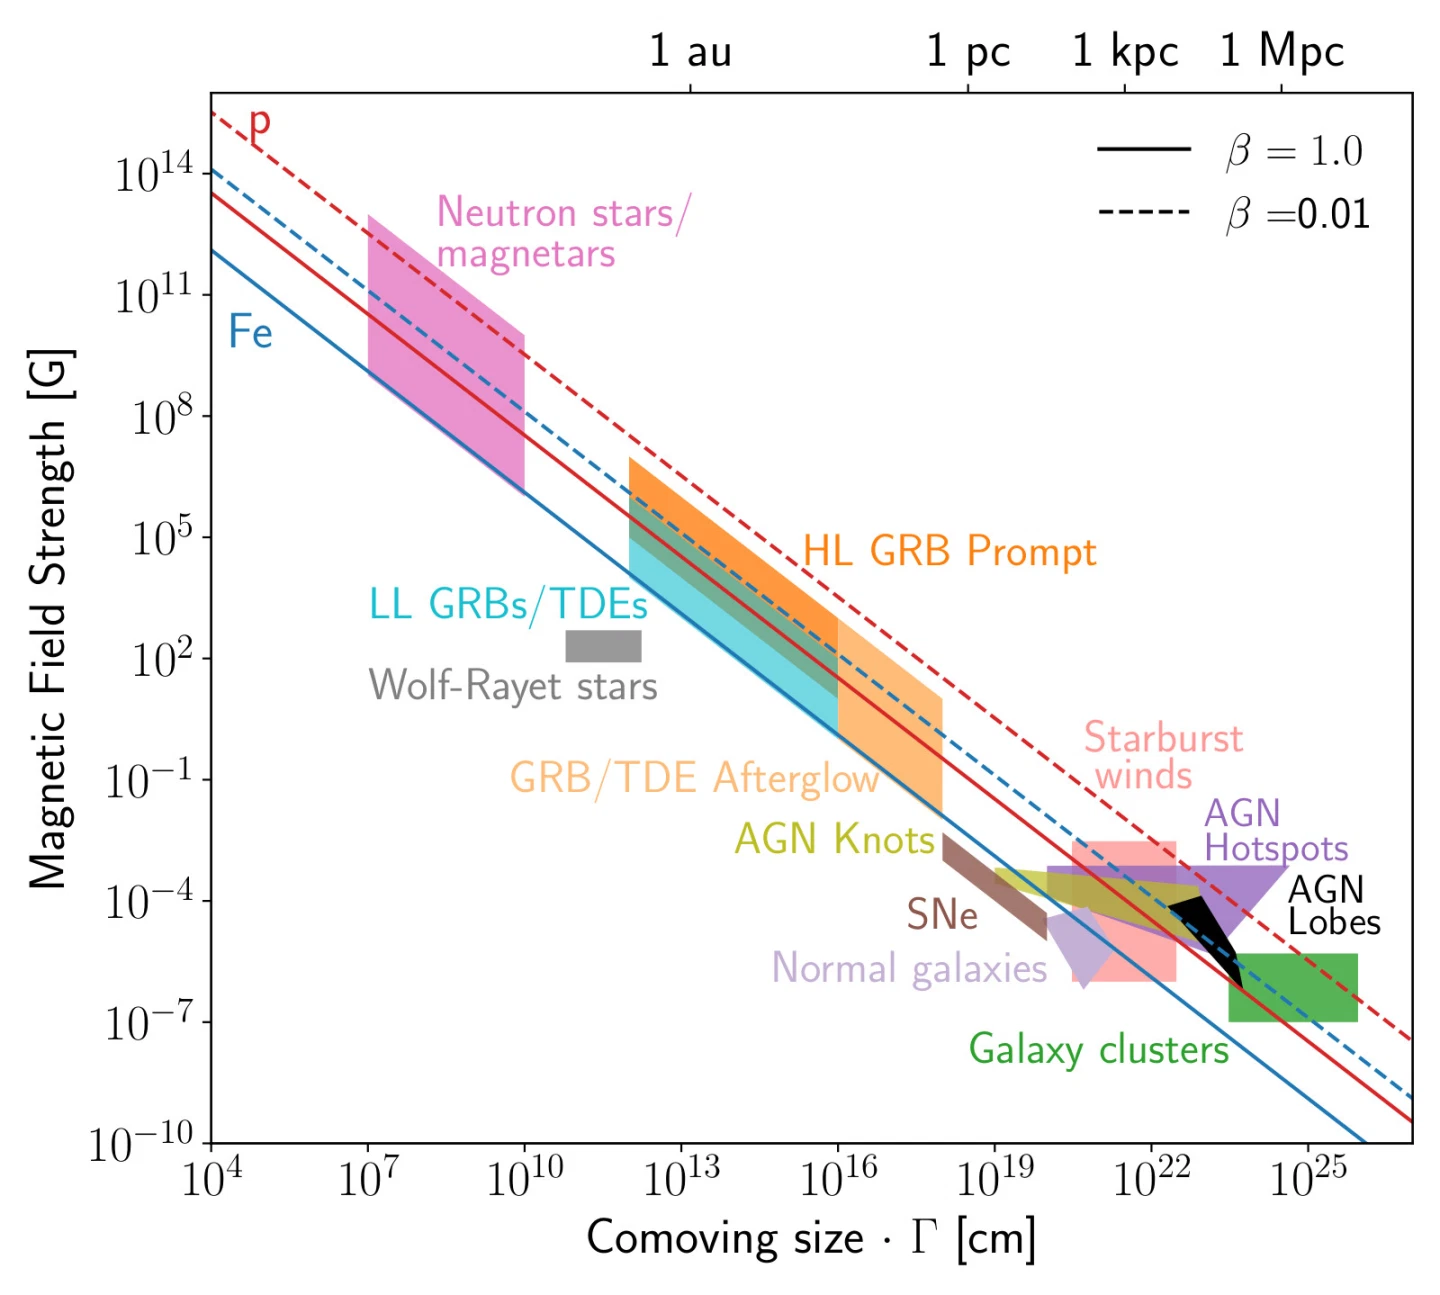
\includegraphics{mma/hillas}
	\caption{A Hillas plot illustrating possible cosmic-ray accelerators. credit: Mauricio B.}
	\label{fig:hillas_plot}
\end{figure}

\section{Neutrinos}

The neutrino was first proposed as a particle by Pauli in 

Solar neutrinos

SN1987A

\emph{Astrophysical neutrinos} are to some degree guaranteed as a byproduct of high-energy cosmic ray production, resulting via pion production from the interaction of cosmic rays with ambient matter (pp) and radiation (p$\gamma$). However, the extent of astrophysical neutrino production depends very substantially on the conditions at cosmic ray accelerators, with high fluxes requiring abundant target material for pion production.

\begin{figure}[!ht]
	\centering 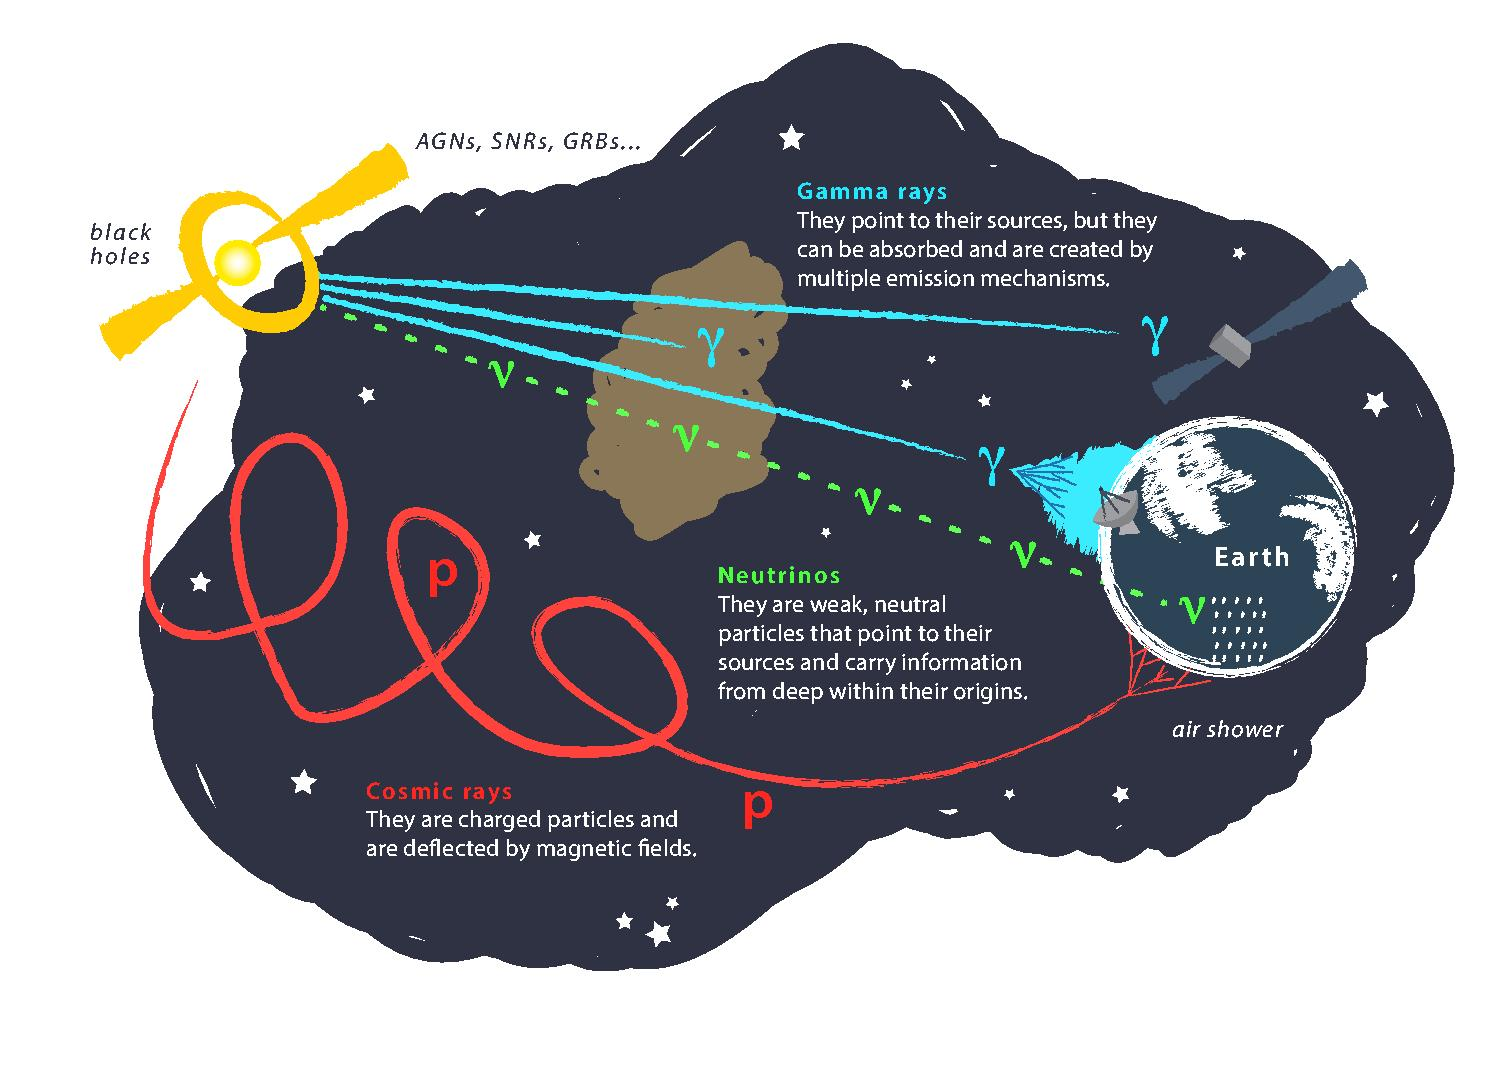
\includegraphics{mma/mm}
	\caption{An overview of multi-messenger astronomy. credit: IceCube.}
	\label{fig:mm}
\end{figure}

In all cases, neutrino production is accompanied by a flux of pionic gamma-rays. However, these can be subsequently absorbed, so neutrinos may be produced in seemingly gamma-dark sources.

Waxmann-Bachall.

Fermi Acceleration

Oscillations

glashow

Kowalski plot

\section{Gravitational Waves}